\documentclass[
	a4page,
	parskip=full,
	% 12pt
]{scrartcl}
\usepackage[margin=2.5cm, bottom=3cm]{geometry}
\usepackage[UKenglish]{babel}
\usepackage{libertinus, libertinust1math}
\usepackage[sfdefault]{biolinum}
\usepackage{roboto}
\usepackage{amsmath,amssymb,amsfonts,amsthm}
\usepackage{graphicx, wrapfig, marginnote, hyperref}
\usepackage[
	% sorting=none,
	% style=verbose
	% style=numeric-comp, % comp = compressed 4,5,6,7 -> 4-7
	sorting=none,		% Sort by appearance
	% autocite = superscript,
	% backref=true,
	url=true
]{biblatex}
\addbibresource{literature.bib}
\AtEveryBibitem{
	\clearfield{url}
	\clearfield{urlyear}
}

% decrease space after disposition
\RedeclareSectionCommands[
	afterskip=1pt
]{section, subsection, subsubsection}
			
\usepackage[ddmmyyyy]{datetime}
\renewcommand{\dateseparator}{.}

\begin{document}

{
	\sffamily\noindent
	Leon Oleschko \hfill \today\\
	Modeling Quantum Hardware: open dynamics and control \hfill Universität Konstanz\\
	\vspace*{1cm}\\
	\textbf{\Large Noise Analysis in an Optomechanical Resonance Cavity}
}

\section*{Project Proposal}
\begin{wrapfigure}{R}{3.5cm}
	\includegraphics{figures/drawing.pdf}
\end{wrapfigure}
Inspired by the noise modelling presented in a proposal for a gravitational antenna \autocite{rainer_weiss_electronically_1972},
I would like to perform a similar analysis of a noise limited experiment.
Specifically, this project will examine the standart quantum limit of a optomechanical resonance cavity using the numerical tools introduced in this course.\\
The modelled setup consists of an optical resonator, with a harmonically moving mirror.
The mirror is thermally coupled to the environment.
Light is coupled into the system as a coherent state, and coupled out to measure the phase.
This introduces shot noise and back action noise in addition to the thermal noise.
These sources are known as the standart quantum limit.

The system Hamiltonian $H$ can be written as a can be written as a combination of the optical and mechanical oscillators.
The optical cavity oscillates with the frequency $\omega_\text{opt} + G \hat x$, where $\hat x$ depends on the position of the mirror position.
The mechanical oscillation is modelled harmonically with $\omega_\text{mech}$.
Therefore the Hamiltonian can be written as a harmonic and a mixing part:
$$
	H_0 = \underbrace{
		a^\dagger a\; (\omega_\text{opt} + G \hat x)
	}_{\text{optical}}+ \underbrace{
		b^\dagger b\; \omega_\text{mech}
	}_{\text{mechanical}}
	= 
	\underbrace{
			a^\dagger a\; \omega_\text{opt}
		+ b^\dagger b\; \omega_\text{mech}
	}_{\text{harmonic}}
	+ 
	\underbrace{
		g\; a^\dagger a\; (b^\dagger + b)
	}_{\text{mixing}}
$$ 

Then using the Lindblad jump operators thermal noise, a driving laser and the measurement can be modelled.
The thermal noise can be modelled in the same way it was done in the lecture.
The driving laser has the effect of adding a coherent state in every time step.
The phase can be measured in a way that introduces radiation pressure into the mechanical oscillator, this is discussed in \autocite{aspelmeyer_cavity_2014}.\\
Modelling a quantum system using a Hamiltonian and Lindblad jump operators is a common technique, that was also discussed in the lecture.
Many numerical implementations for this framework exist, here \textit{QuantumOptics.jl} will be used.\\
With this the standart quantum limit can be explored, with varying system parameters.
This is a combination of Shot Noise, radiation pressure and thermal noise.
This will result in digrams like this:
\begin{center}
	\includegraphics[width=.3\textwidth]{figures/a.png}
	\includegraphics[width=.3\textwidth]{figures/b.png}\\
	From \autocite[FIG. 22]{aspelmeyer_cavity_2014}.
\end{center}

\sloppy
\printbibliography

\end{document}
